% !TeX spellcheck = en_US
\section{Editable isf table}\label{section:isf-table}

In this section we will describe isf table edition window.

Learning and test data tables are stored in isf files. Columns represents objects attributes and rows represents examples of objects. RUDE application support full table edition from UI level. To open editable isf file, you need to double click on isf file in workspace. Isf file with is not editable, represents \hyperref[sub:pct-isf]{Partial Pairwise Comparison Table}. In this chapter we describe only editable isf table.

\begin{figure*}[!ht] 
	\centering
	\makebox[\textwidth]{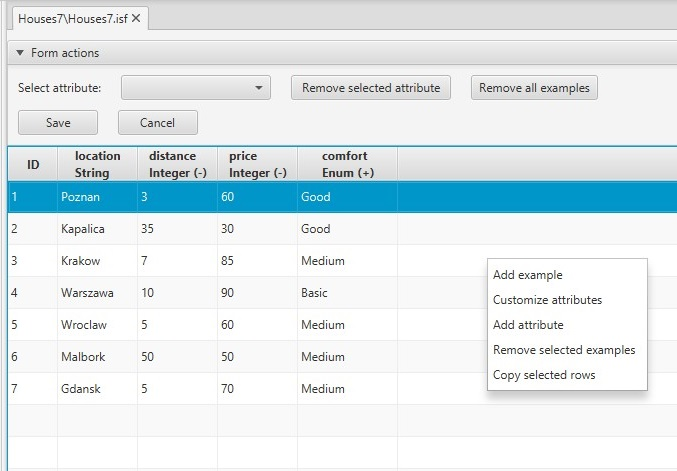
\includegraphics[width=.6\paperwidth]{raw/isf-file}}
	\caption{Isf table edition window for Houses7 experiment}
\end{figure*}

On top of the window, there is expandable panel with form actions.
You can remove attribute (column) from there, if you select attribute in ComboBox and click on Remove selected attribute button. You can also clear table by removing all examples.

Below actions panel you can see editable isf table. In table header attribute name, type and cost (-)/gain (+) criterion is displayed. If you hover over column header additional information will be presented in tooltip. ID column is generated by application and it is used only to provide row number. It is not saved in isf file. Table columns can be also colored, when they are inactive (red) or are decision attributes (green).

\subsection{Table edition}\label{sub:isf-examples}

You can reorder attributes (columns) freely. You can also sort values in attributes. This changes will be saved to isf file.

You can edit examples by double clicking on cell in table. Changes will be saved after pressing Enter button or clicking on other cell. Edition will be canceled after pressing Escape button.

Each field type allows different set of characters:
\begin{itemize}
	\item \textbf{String} - stores alphanumerical text, mostly used for description attributes.
	\item \textbf{Integer} - stores integer values.
	\item \textbf{Cardinal} - stores positive integer values.
	\item \textbf{Decimal} - stores floating point values, scientific notation is supported here.
	\item \textbf{Enum} - stores text values with are selectable from list.
\end{itemize}

Table supports context menu actions. Context menu can be opened by right clicking on table. It contains following actions:
\begin{itemize}
	\item \textbf{Add example} - adds new empty example (row).
	\item \textbf{Customize attributes} - opens modal dialog for editing attributes (columns).
	\item \textbf{Add attribute} - opens modal dialog for adding new attribute.
	\item \textbf{Remove selected examples} - remove selected examples (rows) from table. Multi-select is enabled.
	\item \textbf{Copy selected rows} - exports selected rows to CSV format. Attribute (columns) names will be used for header. Exported rows will be copied to user clipboard.
\end{itemize}

\subsection{Adding new attribute}\label{sub:isf-add-attr}

New attribute can be added by choosing ''Add attribute'' option from context menu. All fields are required in this form.

\begin{figure*}[!ht] 
	\centering
	\makebox[\textwidth]{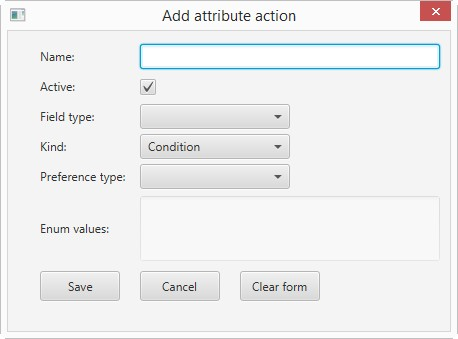
\includegraphics[width=.4\paperwidth]{raw/isf-add-attr}}
	\caption{Add new attribute dialog}
\end{figure*}

Field type was described earlier in \hyperref[sub:isf-examples]{Table edition section}. By default, field is active, with means that it is not excluded from experiment.
If attribute condition type will be selected, attribute will be used in experiment as normal field. If decision type was selected and has gain/cost preference type, it can be used to calculate reference ranking from examples in isf table. It will be used when running experiment. 
\\ Description field kind is not used in experiment and serves only for informational purposes. Preference type is used to determine if values in field have cost or gain criterion. Enum values field is only used for enum field type. If enum field type is chosen, list of values can be provided there by separating them by comma.

\subsection{Customizing existing attribute}\label{sub:isf-cust-attr}

Existing attributes (columns) can be edited by choosing ''Customize attributes'' option from context menu.

\begin{figure*}[!ht] 
	\centering
	\makebox[\textwidth]{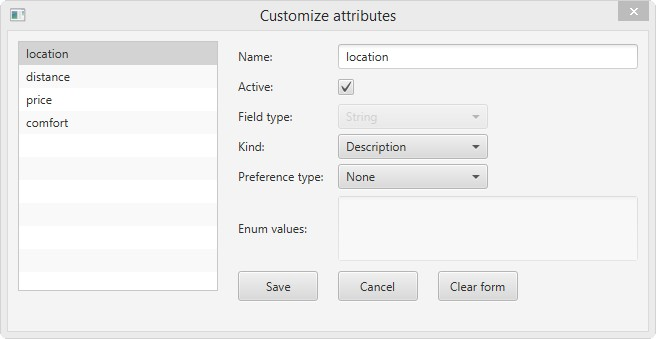
\includegraphics[width=.6\paperwidth]{raw/isf-customize-attr}}
	\caption{Customize attributes dialog}
\end{figure*}

Form in this dialog is similar to ''Add attribute'' dialog. Field type is disabled to avoid conversion problems between attributes, like conversion from string to integer. On the left side of dialog, you can choose attribute to edit. Changes in all attributes will be saved after clicking on save button.


\vfill\newpage